%卒業論文用テンプレート
\documentstyle[graphicx]{jronbun}


%諸定義
\newenvironment{indention}[1]{\par
\addtolength{\leftskip}{#1}
\begingroup}{\endgroup\par}

%論文名
\title{マルチサイクルテストにおける遅延故障の検出強化技術}
%教官名
\kyoukan{高橋寛教授}
\second{王森レイ講師}
%名前
\author{長滝谷剣}
%提出日
\date{令和3年2月15日提出}
%講座名
\kouza{\gt 愛媛大学工学部情報工学科情報システム工学講座}

\begin{document}
%タイトル生成
\maketitle
%目次生成
\pagenumbering{roman}
\tableofcontents
\cleardoublepage
\pagenumbering{arabic}

%--ここから本文-----------------------------------
%第1章 まえがき
\chapter{まえがき}
%まえがき

%1節
\section{研究背景}
近年,航空機や自動運転などにのシステムの機能安全を保障するために,
半導体デバイスの運用時に故障の有無を検査するフィールドテストが求められる.
パワーオンセルフテスト(POST)は、一つの代表的なフィールドテスト技術である.
POSTはシステムの起動時にデバイスに対して検査を行い,
短時間(システムの起動時間,およそ数十ms)により多くの故障を検出する必要がある.
そのため,より検出精度の高い手法を求め研究が行われている.

故障検出手法の1つにマルチサイクルテスト\cite{multicycle}がある.
マルチサイクルテストは,キャプチャ動作時に複数回のキャプチャサイクルを与えることで,
各サイクルで得られた値を次のキャプチャサイクルのテストパターンとして再利用する手法であり,
従来のテスト手法と比較して,より多くの故障検出の機会が与えられるため,POSTの性能向上に有効な手法である.

%2節
\section{研究目的・目標}
本研究の目的は,システムの機能安全保障のために,
マルチサイクルテストを用いたPOSTにおける遅延故障に対する検出能力を向上することである.

先行研究では,マルチサイクルテストにおける縮退故障の検出モデルを解析し,
縮退故障の検出能力を向上するために回路内に故障を容易に検出できるようなテスト容易化技術を提案した.
しかしながら,遅延故障は時間に関わる故障であり,故障の検出方式は縮退故障と異なるため,
マルチサイクルテストによる遅延故障に対する検出効果が明確ではない.
そこで,本研究の目標は,マルチサイクルテストにおける遅延故障のテスト方法について検討し,
その検出効果を評価する.さらに,マルチサイクルテストにおける遅延故障の検出能力を向上するために,
一部のFFにキャプチャ後の値を強制的に反転させるFF制御回路を挿入するFF-CPI技術を導入し,
その効果を評価する.

%3節
\section{本論文の構成}
本論文は以下のような構成となっている.
第1章では,本研究に至った背景や研究目的,目標について述べる.
第2章では,本論文を閲覧するにあたり必要となる用語について,
第3章では,マルチサイクルテストの概要及びマルチサイクルテストの利点と欠点について述べる.
第4章では,FF制御について述べる.
第5章では,本研究における実験内容及び実験結果について述べ,
第6章では,実験に対する評価,考察を述べる.
また,第7章では,本研究を通してのまとめを記載している.


%第2章 定義
\chapter{定義}
%定義
本章では,本論文を閲覧するにあたり必要となる用語について述べる.

%1節
\section{スキャンテスト}
スキャンテスト\cite{scantest}とは,組み合わせ回路にFFを取り付けることで,
回路のテストや内部状態の制御・観測を容易にしたテスト手法である.
スキャンテストの構成を図2.1に示す.
\begin{figure}[]
	\begin{center}
		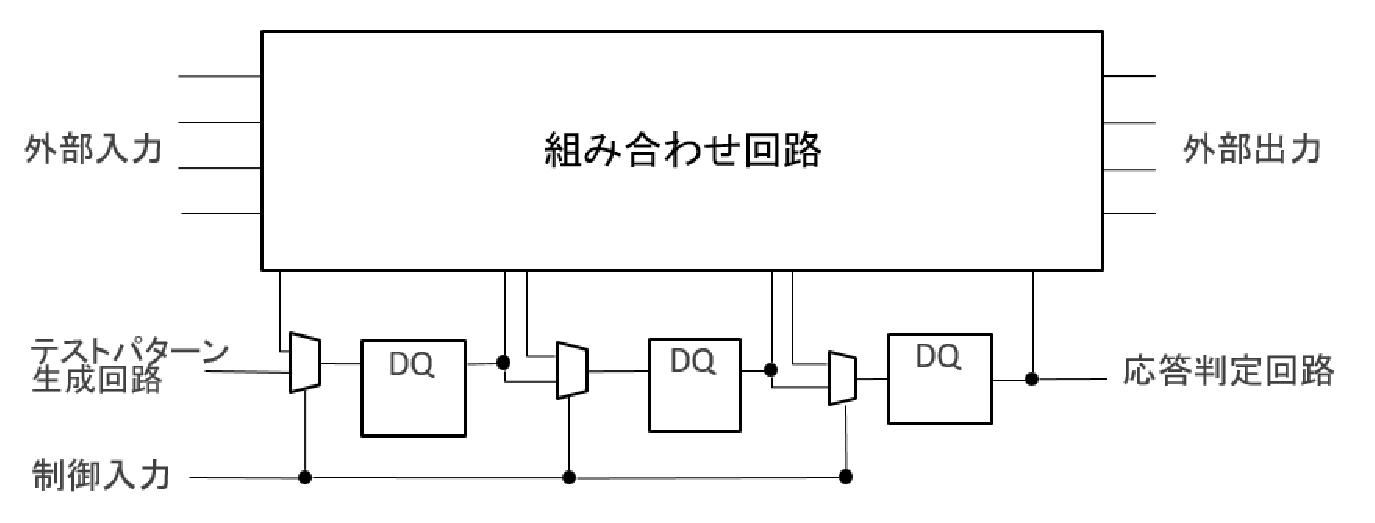
\includegraphics[height=50mm]{scantest.eps}
		\caption{スキャンテスト}
	\end{center}
\end{figure}

対象となる順序回路のFFを,
直列につないだシフトレジスタ(スキャンチェーン)に置き換え,
スキャン出力まで値をシフトし内部状態の制御・観測を行う.
また,テストパターン生成回路とテスト応答判定回路を組込むことで簡易的な検査が可能となる.
テストパターン生成回路には線形帰還シフトレジスタ(LFSR: Linear Feedback Shift Registe)
がよく用いられる.本研究でもLFSRを用いた回路を想定している.
スキャンテストはシフトモードとキャプチャモードによってテストを行う.
シフトモードとは,スキャンインと呼ばれるLFSRが生成したテストパターンを各FFに印加する動作と,
スキャンアウトと呼ばれる結果の出力を行う動作の二つの動作を持つモードである.
キャプチャモードとは,スキャンチェーンに印加したテストパターンを用いて
回路の応答をFFにキャプチャするモードである.

%2節
\section{遅延故障}
論理回路内の素子や信号線における信号変化の伝搬遅延時間が増大し
誤作動を起こす故障を遅延故障\cite{transfault}と呼ぶ.
遅延故障の故障モデルを図2.2に示す.
図に示すように,FFの出力で生じた信号値変化が
組み合わせ回路内を伝搬して次のクロックでFFに取り込まれる際,
遅延時間が決められた範囲を超えることで誤作動が生じる.
遅延故障には,立ち上がり(0から1への変化)の遅延と,
立ち下がり(1から0への変化)の遅延の二通りの故障が考えられる.

\begin{figure}[h]
\begin{center}
	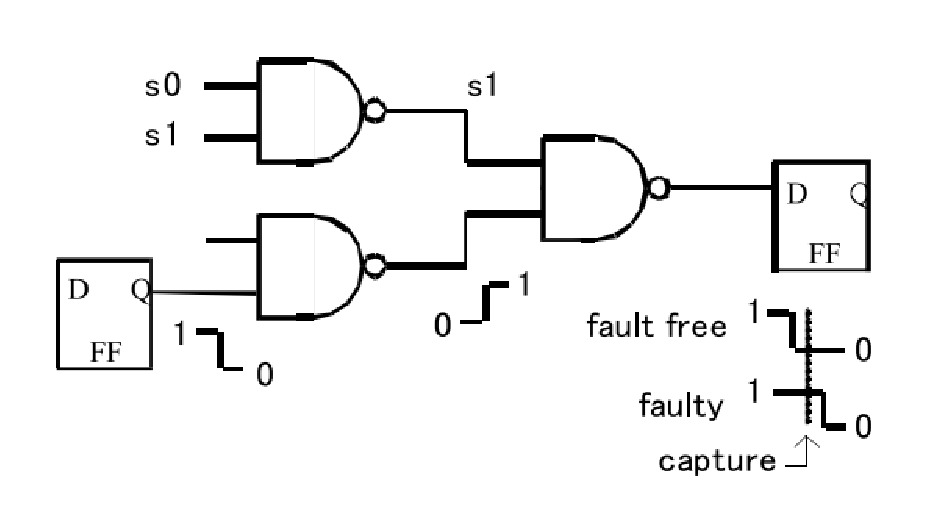
\includegraphics[height=50mm]{transfault.eps}
	\caption{遅延故障モデル}
\end{center}
\end{figure}

%3節
\section{遅延故障のテスト方式}
遅延故障は信号値の変化に起因することから,故障を検出するためには,
変化前の信号値を設定するためのテストパターンと,
変化後の値をキャプチャするためのテストパターンの2つを連続して印加する必要がある.
この手法を2パターンテストと呼ぶ.

2パターンテストで高い故障検出率を得るためには,テストパターンの印加方法を工夫する必要がある.
スキャン動作は,1パターン目の印加と2パターン目の出力の観測に有効であるが、
1パターン目と2 パターン目を連続して実動作時間で印加することができないためである.
この問題を解決する手法の一つとして,次節で説明するラウンチオフキャプチャ方式
(LoC : Launch off Capture)が存在する.

%4節
\section{LoC方式}
LoC方式\cite{transfault}では,スキャンシフト動作で1パターン目をスキャンチェーンに設定した後,
通常動作で, システムクロックにより2パターン目を設定し,続けてキャプチャを行う.
つまり,スキャンインをした後に,システムクロックにより二回キャプチャを行うことになる.
図2.3にクロック信号とスキャンイネーブル信号のタイミングチャートを示す.

\begin{figure}[h]
	\begin{center}
		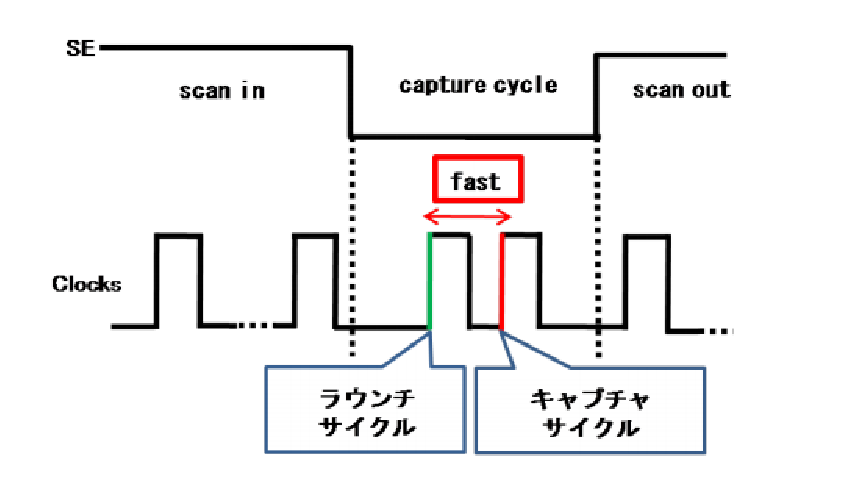
\includegraphics[height=50mm]{LoC.eps}
		\caption{LoCのタイミングチャート}
	\end{center}
\end{figure}

LoC方式の特徴として,2パターン目が通常動作と同じなので設計時の制約が少ないことがあげられる.
また,正常な回路を不良と判定する歩留まりの低下の危険性も少ないこともあげられる.

%本研究では,LoC方式に対して図2.4に示すようにマルチサイクル化を施す.


%第3章 
\chapter{マルチサイクルテスト}
%マルチサイクルテスト
本章では,マルチサイクルテストの概要と,
マルチサイクルテストにおける縮退故障の検出および遅延故障の検出に関してそれぞれ述べる.

%1節
\section{マルチサイクルテスト}
マルチサイクルテスト\cite{multicycle}とは,スキャンテストにおいて
複数回のキャプチャサイクルを繰り返す手法である.
LoC方式に対してマルチサイクル化を施した場合のタイミングチャートを図3.1に示す.

\begin{figure}[h]
	\begin{center}
		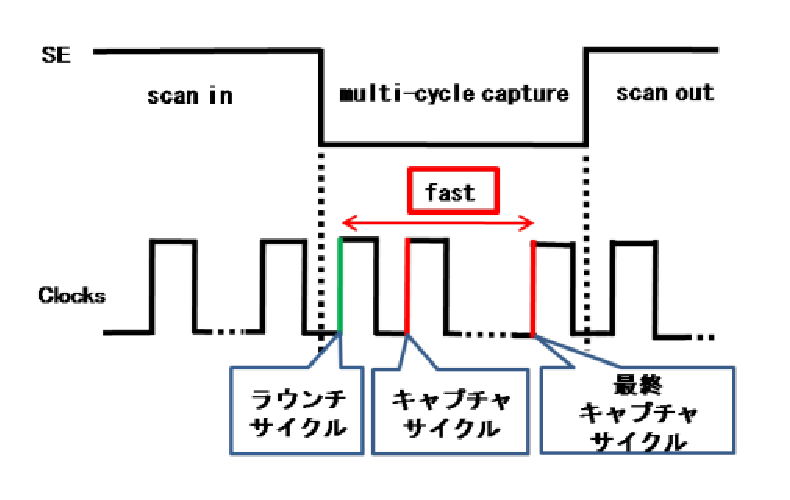
\includegraphics[height=50mm]{LoCmulti.eps}
		\caption{マルチサイクルによるLoCのタイミングチャート}
	\end{center}
\end{figure}

マルチサイクルテストでは,スキャンシフト動作でテストパターンをスキャンチェーンに設定した後,
通常動作で,システムクロックによりキャプチャを行い,テスト応答としてスキャンチェーンに値が設定される.
その後,2サイクル目のテストモードにおいて,再度キャプチャを行い,
テスト応答がスキャンチェーンに設定される.
このように,キャプチャを繰り返し最終キャプチャで得られた値をスキャンアウトすることで,
テストパターンに対するテスト応答を確認する手法である.

マルチサイクルテストの時間実行例としてサイクル数を3とした場合の例を図3.2に示す.
まず,スキャンイン動作で(110)が入力される.
1サイクル目でキャプチャされたパターン(001)を入力として2サイクル目が実行される.
2サイクル目でキャプチャされたパターン(101)を入力として3サイクル目が実行される.
3サイクル目でキャプチャされたパターン(101)をスキャンアウトすることでテスト結果を得る.

\begin{figure}[h]
	\begin{center}
		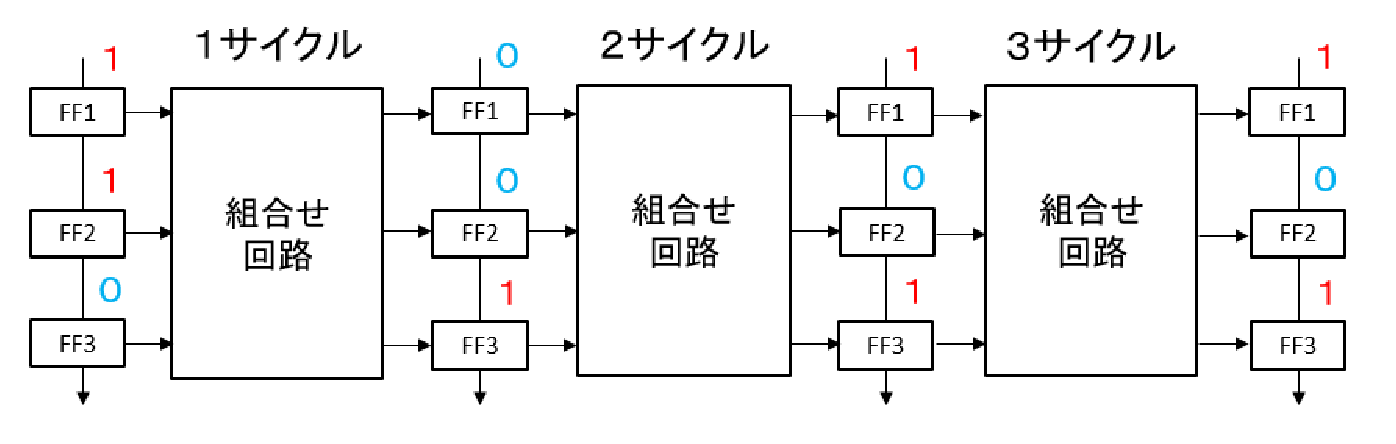
\includegraphics[height=40mm]{multicycle.eps}
		\caption{マルチサイクルテスト}
	\end{center}
\end{figure}	

マルチサイクルテストでは,各サイクルでキャプチャされたパターンを
次のキャプチャサイクルのテストパターンとして再利用することで,
従来のスキャンテストと比較したときに,テストパターンの生成数を抑えつつ
より多くの故障検出を行う機会を獲得できる.

%2節
\section{マルチサイクルテストにおける故障検出}

%2節1項
\subsection{マルチサイクルテストにおける縮退故障の検出}
ここでは,マルチサイクルテストにおける縮退故障の検出に関して述べる.
ある信号線Lの0(1)縮退故障を検出するためには,
テストパターンによってその信号線Lに1(0)を設定することで故障が励起される.
次に,この縮退故障の影響が被検査回路の出力側のフリップフロップにおいて
誤り論理値として取り込まれることによって,
テストパターンによって縮退故障が検出できたと判定する.

図3.3にマルチサイクルテストにおける縮退故障の検出例を示す.

\begin{figure}[h]
	\begin{center}
		\includegraphics[height=70mm]{degenetest.eps}
		\caption{マルチサイクルテストにおける縮退故障の検出例}
	\end{center}
\end{figure}

マルチサイクルテストにおいては,まず,
スキャンフリップフロップにテストパターンがスキャンインされた後に,
被検査回路をシステムクロックのテストモードで動作させる.
次に,キャプチャクロックで1サイクル目のテストモードで回路が動作した結果として,
得られた応答がフリップフロップに取り込まれる.
図3.2の例では,2サイクル目以降のフリップフロップにおいて,
テスト時に取り込まれた論理値と期待値が異なるため,
最終サイクルのテストモードにおいて回路が動作した結果として
得られた応答がフリップフロップに取り込まれ,
テスト時に取り込まれた論理値と期待値が異なるため縮退故障が検出できたと判定する.

%2節2項
\subsection{マルチサイクルテストにおける遅延故障の検出}
ここでは,マルチサイクルテストにおける遅延故障の検出に関して述べる.
ある信号線Lの立ち下がり(立ち上がり)遅延故障を検出するためには,
まず,テストパターンによってその信号線Lに1(0)を初期値として設定し,
次のテストパターンによってその信号線Lに0(1)を設定することで,
立ち下がり(立ち上がり)遅延故障が励起される.
次に,この遅延故障の影響が被検査回路の出力側のフリップフロップにおいて
誤り論理値が取り込まれることによって,テストパターンによって遅延故障が検出できたと判定する.

図3.4にマルチサイクルテストにおける遅延故障の検出例を示す.

\begin{figure}[h]
	\begin{center}
		\includegraphics[height=70mm]{trantest.eps}
		\caption{マルチサイクルテストにおける遅延故障の検出例}
	\end{center}
\end{figure}

マルチサイクルテストにおいては,まず,
スキャンフリップフロップにテストパターンがスキャンインされた後に,
被検査回路をシステムクロックのテストモードで動作させる.
次に,キャプチャクロックで1サイクル目のテストモードで回路が動作した結果として,
対象とする信号線に初期値を設定している.
次に,2サイクル目のテストモードにおいて,
対象とする信号線に信号遷移(立ち上がり信号変化)を励起している.
対象とする信号線の信号遷移(立ち上がり信号変化)が遅延故障の影響を受けるので,
その遅延故障の影響が伝搬する出力側のフリップフロップにおいて誤り論理値が取り込まれる.
その誤り論理値の影響が最終サイクルまで伝搬することによって,遅延故障が検出できたと判定する.

さらに,図3.4では,4サイクル目に初期値1を設定し,
5サイクル目で対象とする信号線に信号遷移(立ち下がり信号変化)を励起し,
出力側のフリップフロップにおいて誤り論理値が取り込まれることで,遅延故障が検出できたと判定する.

%3節
\section{マルチサイクルテストにおける故障検出能力低下問題}
マルチサイクルテストには ``故障検出能力低下問題'' がある.
故障検出能力低下問題\cite{multidemerit}とは,キャプチャサイクルを重ねるにつれ
次第に新たな故障を検出しにくくなっていく問題である.
マルチサイクルテストでは,被検査回路の内部状態を機能動作に近づけることができ,
多数のキャプチャサイクル(20サイクル)を適用した場合,
被検査回路の内部状態遷移はサイクル数を増やすことによって低減することが報告されている\cite{FFtgl}.
多数のキャプチャサイクルを適用した場合における,
FFの内部状態遷移を示したグラフを図3.5に示す.
図の縦軸は,各FFの値がサイクル毎に遷移の発生した回数,横軸はサイクル数を示している.

\begin{figure}[h]
	\begin{center}
		\includegraphics[height=70mm]{FFtgl.eps}
		\caption{マルチサイクルキャプチャによるFFの状態遷移回数変化(s298ベンチマーク回路)}
	\end{center}
\end{figure}

図から読み取れるように,サイクル数の増加に伴い各FFの内部状態の遷移回数は減少することから,
多数のキャプチャサイクルを適用した場合,FFの値は固定値となり,故障検出能力は低下する.

故障検出能力低下問題におけるFF固定値の例として,
サイクル数を3とした場合のマルチサイクルテストを図3.6に示す.

\begin{figure}[h]
	\begin{center}
		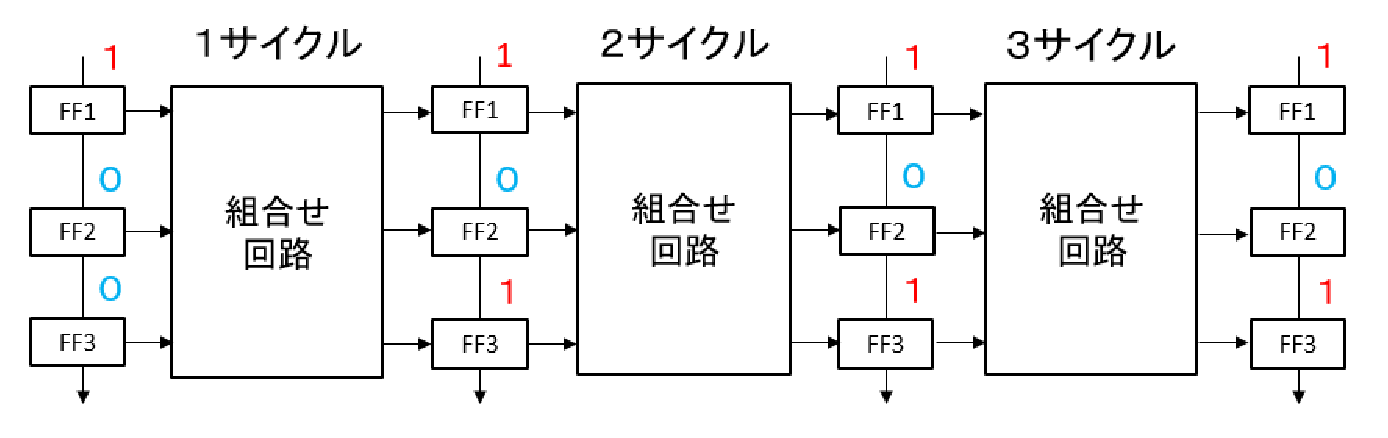
\includegraphics[height=40mm]{trandem.eps}
		\caption{マルチサイクルテストにおける故障検出能力低下問題}
	\end{center}
\end{figure}

まず,スキャンイン動作で(100)が入力される.
1サイクル目でキャプチャされたパターン(101)を入力として2サイクル目が実行される.
2サイクル目でキャプチャされたパターン(101)を入力として3サイクル目が実行される.
3サイクル目でキャプチャされたパターン(101)をスキャンアウトすることでテスト結果を得る.

このように,被検査回路の内部状態遷移の減少によって,
キャプチャパターンが最初のサイクルで適用されたテストパターンと比較して,
ランダム性の少ない入力パターンになってしまい,
新たな故障を検出する能力が低下する.
この問題を改善し,故障を検出する能力を向上させるため,
4章で説明するFF制御点挿入を用いて実験を行う.

%第4章
\chapter{FF制御点挿入技術(FF-CPI)}
%FF制御
本章では,マルチサイクルテストにおける故障検出能力低下問題への対策として,
FF制御点挿入技術(FF-CPI)について述べる.

%1節
\section{故障検出能力低下問題への対策}
3章で説明したように,マルチサイクルテストでは,キャプチャサイクルの増加に伴い,
被検査回路の内部状態遷移が低減し,新たな故障の検出が困難になる問題がある.
この対策として,文献[5]では,
FFの出力に値を強制的に遷移させる制御ポイント(CP)を挿入するFF-CPI技術が提案された.
制御ポイント挿入技術とは,被検査回路の内部状態遷移の低減によって
故障信号の伝搬や励起を阻害しているFFに,直接論理値を割り当てる技術である.
FFにCPを挿入することで,制御後のサイクルにおける
キャプチャパターンのランダム性を向上させることができる.
固定値0/1が印加される箇所に対して,制御した論理値1/0を割り当てることにより,
故障の励起を促し,故障検出能力の向上を期待する.

%2節
\section{FFCP回路構造}
本研究では,FFトグリング制御を用いる.
トグリング制御の制御モデルを図4.1に示す.

\begin{figure}[h]
    \begin{center}
        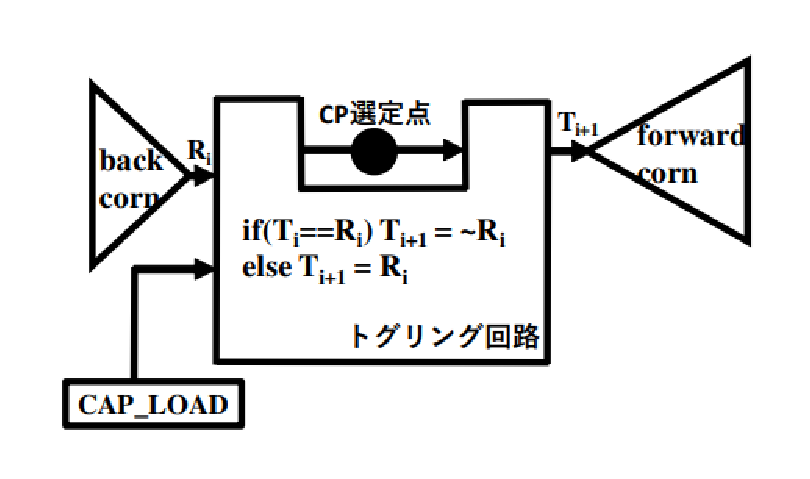
\includegraphics[height=50mm]{tgl.eps}
        \caption{トグリング制御モデル}
    \end{center}
\end{figure}

トグリング制御とは,選定した信号線にトグル回路を追加することで,
サイクル毎に選定信号線の値をトグルさせる手法である.
キャプチャモードでは,現在の状態(Ti:現在のキャプチャサイクルで適用されたテストパターン)と,
次の状態(Ri:現在のキャプチャサイクルで適用されたテストパターンのレスポンス)を比較して,
FFの値が変化しているかを確認する.変化していない場合は,
トグル制御回路はTi+1にトグルを生成し,Riの反転値を次のサイクルに伝搬させ,
変化している場合は,ば次のサイクルに現在のRiを伝搬させる.

また,本実験では,FF制御箇所はランダムに選定する.


%第5章
\chapter{実験}
%実験・結果
本章では,本研究における実験内容及び結果について述べる.

%1節
\section{実験内容}
遅延故障シミュレータにFF制御を実装し,検出率を算出する.
本実験では,全体の10\%のFFを制御した.
FF制御を行う場合と行わない場合それぞれにおいて,
遅延故障検出率の観点から性能差を比較する.
今回実験に用いた回路の詳細は表5.1の通りである.
\begin{table}[htb]
 \begin{center}
 \caption{実験回路情報}
  \begin{tabular}{|l|r|r|r|} \hline
    回路名 & s5378 & s9234 & s13207 \\ \hline \hline
    信号線の数 & 5344本 & 9256本 & 13300本 \\
    FFの総数 & 179個 & 228個 & 669個 \\
    制御するFFの数 & 17個 & 22個 & 66個 \\ \hline
  \end{tabular}
  \end{center}
\end{table}

3種類すべての回路において,テストパターン数100でシミュレーションを行い,
2サイクルから10サイクルにかけての遅延故障検出率の推移を算出した.
なお,本研究で使用されたプログラムはすべてC言語で開発されている.

%2節
\section{実験結果}
それぞれの回路における遅延故障検出率を以下の図に示す.
図では,FF制御なしのグラフは青線で,FF制御ありのグラフは黄線で表している.
得られた結果に対する考察は次章にて述べる.

\begin{figure}[h]
\begin{center}
	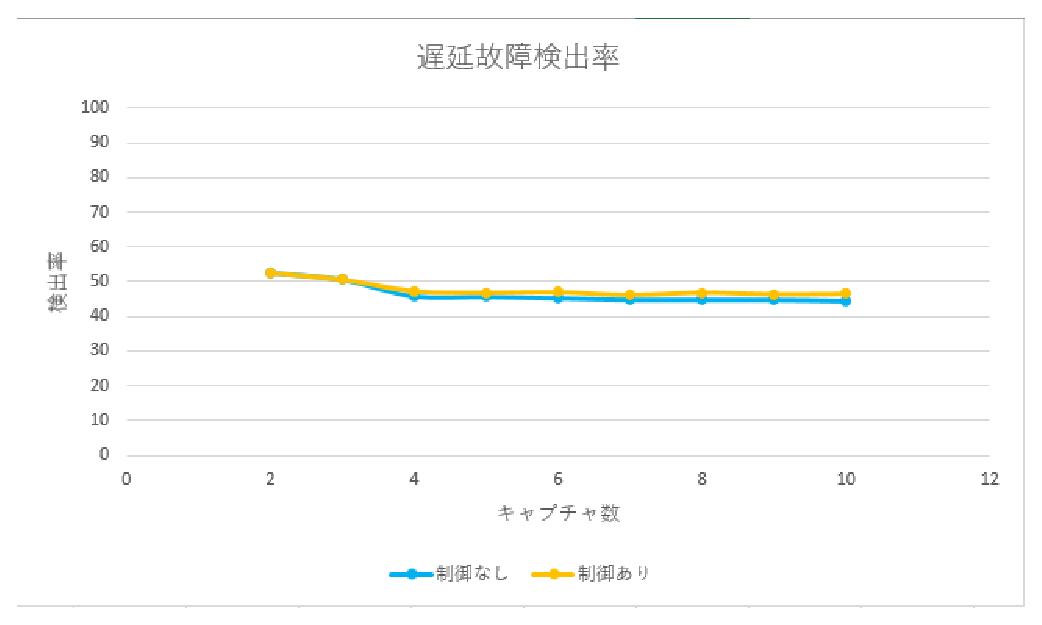
\includegraphics[height=80mm]{s5378CPI.eps}
	\caption{s5378回路における遅延故障検出率}
\end{center}
\end{figure}

\begin{figure}[h]
\begin{center}
	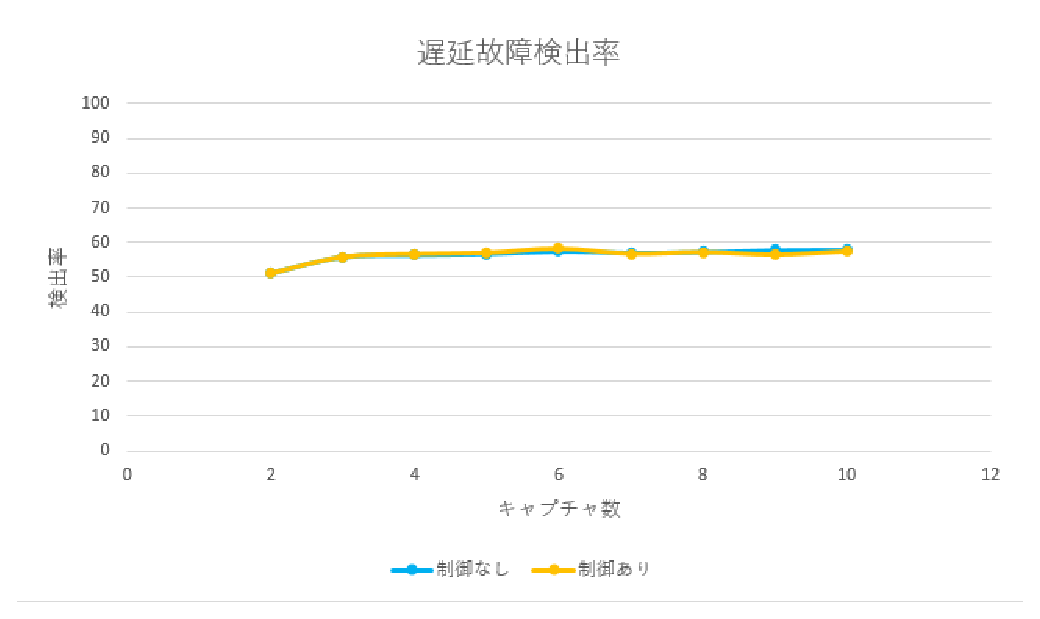
\includegraphics[height=80mm]{s9234CPI.eps}
	\caption{s9234回路における遅延故障検出率}
\end{center}
\end{figure}

\begin{figure}[h]
\begin{center}
	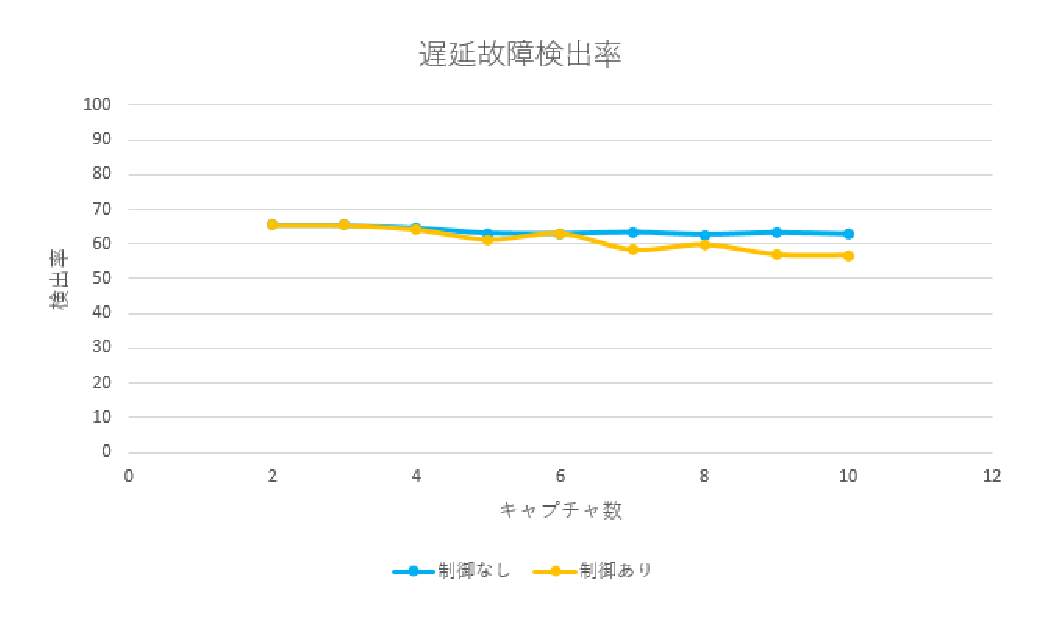
\includegraphics[height=80mm]{s13207CPI.eps}
	\caption{s13207回路における遅延故障検出率}
\end{center}
\end{figure}

%第6章
\chapter{考察}
%考察
本章では,実験結果に対する考察について述べる.

%\section{評価・考察}
マルチサイクルテストにおける遅延故障検出結果として,
キャプチャ数を増やすと故障検出率が低下する傾向にあることが判明した.
この結果は,キャプチャ数を増加させるにつれて内部状態が次第に遷移しなくなるという,
``故障検出能力低下問題''に起因する可能性が高い.
また,s9234回路に関してのみ,キャプチャ数の増加に伴い故障検出率が増加しているが,
これは回路そのものが原因であると推測する.

FF制御を行った場合の実験結果では,
s5378回路では,ほとんどのキャプチャ数において故障検出率が1.5\%程度向上し,
s9234回路では,いくつかのキャプチャ数において故障検出率が0.8\%ほど向上したことが明らかとなった.
しかしながら,s13207回路においては,ほとんどのキャプチャ数において故障検出率が悪化する結果となり,
FF制御が遅延故障検出率の向上に必ずしも寄与するとは言い難い結果となった.
回路ごとに最適なCP挿入箇所が存在するものの,本実験ではCP挿入箇所をランダムに選定したことが,
今回の得られた結果の原因である可能性が高い.
CP挿入箇所選定手法に関して,より適した選定点の提案を実現できれば,
遅延故障検出率を向上させることができる.

%第7章
\chapter{まとめ}
%まとめ

%\section{今後の課題}
本研究では,マルチサイクルテストが遅延故障検出率にどのような結果をもたらすのか検証した.
実験では,外部から直接論理値を割り当てるCPをFFに挿入する手法を提案し,
FF制御の有無で,遅延故障検出率の性能差を算出した.
結果からは,提案手法により,わずかながら故障検出能力の向上が確認できた.

今後の課題として,FFCPの選定位置の最適化が挙げられる.
現在は選定位置はランダムとしているが,より適した位置にCPを挿入することで,
遅延故障検出率を更に向上させる必要がある.
%--ここまで本文-----------------------------------


%謝辞
\newpage
\addcontentsline{toc}{chapter}{\protect\numberline{謝辞}{}}
\chapter*{謝辞}
%--ここから謝辞--
本研究を進めるにあたり,
懇篤な御指導,御鞭撻を賜わりました本学高橋寛教授に深く御礼申し上げます.

本論文の作成に関し,
詳細なるご検討,貴重な御教示を頂きました本学王森レイ講師ならびに甲斐博准教授に深く御礼申し上げます.

また,本研究に際しご審査いただきました本学井門 俊講師に深く御礼申し上げます.

最後に,多大な御協力と貴重な御助言を頂いた
本学工学部情報工学科情報システム工学講座高橋研究室の諸氏に厚く御礼申し上げます.

%--ここまで謝辞--

%参考文献
\begin{thebibliography}{99}
%ここから参考文献

%--例--
%\bibitem{Interconnect}
%Bram Kruseman , Ananta K. Majihi , Wilmar Heuvalman , Jennifer Dworak“NIM-X : A Noise Index Model-Based X-Filling technique to Overcome the Power Supply Switching Noise Effects on Path Delay Test" IEEE Trans. on VLSI Test Symp. ,pp.809-813, May. 2012.

\bibitem{multicycle}
山口 久登,松薗 誠,佐藤 康夫,梶原 誠司 : 
“スキャンBIST におけるマルチサイクルテストと部分観測方式の提案と評価" ,
電子情報通信学会技術研究報告,DC2010-28,pp.31-36,2010-11 

\bibitem{scantest}
藤原 秀雄 : 
“コンピュータの設計とテスト" ,
工学図書 pp.221,1990

\bibitem{transfault}
梶原 誠司・佐藤 康夫 : 
“論理回路に対する遅延テスト手法" ,
https://www.jstage.jst.go.jp/article/essfr/1/3/1\_3\_3\_71/\_pdf

\bibitem{multidemerit}
J. Rearick, ”Too Much Delay Fault Coverage is a Bad Thing,” Proc. Int ’l Test
Conf., Baltimore, MD, pp. 624-633, 2001. DOI: 10.1109/TEST.2001.966682

\bibitem{FFtgl}
Hanan T. Al-AWADHI, Tomoki AONO, Senling WANG, Yoshinobu HIGAMI, 
Hiroshi TAKAHASHI, Hiroyuki IWATA, Yoichi MAEDA, Jun MATSUSHIMA, 
”FF-Control Point Insertion (FF-CPI) to Overcome the Degradation of Fault Detection under Multi-Cycle Test for POST”,
IEICE Transactions on Information and Systems, 2020, E103.D 巻, 11 号, p. 2289-2301, 
公開日 2020/11/01, Online ISSN 1745-1361, Print ISSN 0916-8532

%ここまで参考文献

\end{thebibliography}
\end{document}
